\subsubsection{Adaptaci�n}
\begin{frame}

\frametitle{Adaptaci�n}

\begin{figure}
\begin{tikzpicture}[node distance=0.5cm, auto,>=latex', thick]
\scriptsize
    % We need to set at bounding box first. Otherwise the diagram
    % will change position for each frame.
    \path[use as bounding box] (-1.5,0) rectangle (12,-2);

    % TT methodology     
    \node [phase]                        (monitoreo)     {Vigilancia};
    \node [phase, below of=monitoreo]    (choice)        {Elecci�n};
    \node [phase, below of=choice]       (acquisition)   {Adquisici�n};
    \node [phase2,below of=acquisition]  (adaptation)    {Adaptaci�n};
    \node [phase, below of=adaptation]   (absortion)     {Absorci�n};
    \node [phase, below of=absortion]    (aplication)    {Aplicaci�n};
    \node [phase, below of=aplication]   (difusion)      {Difusi�n};

    %%%%%%%%%%%%%%%%%%%%%%%%%%%%%%%%%%%%%%%%%%%%&
    %            Adaptaci�n   
    %%%%%%%%%%%%%%%%%%%%%%%%%%%%%%%%%%%%%%%%%%%%&
    \onslide<1> \node [ph_explain, right=.5cm of adaptation.east] (exp_adaptation)    
    {
    \begin{center} \textbf{Adaptaci�n} \end{center}
    \begin{itemize}
     \item Se presenta cuando la sociedad encuentra posible y deseable realizar cambios para involucrar usos particulares de la tecnolog�a.
%        \begin{itemize}
%         \scriptsize
%         \item Adquisici�n de un dispositivo comercial. 
%         \item Aplicar ingenier�a inversa para identificar su arquitectura y forma de programaci�n.
%         \item Generaci�n de aplicaciones similares a la original. 
%         \item Dise�o y construcci�n local.
%         \item Transmisi�n de conocimientos a la academia y a la industria.
%         \item Documentaci�n del proceso a todo sector de la sociedad.
%        \end{itemize}
    \end{itemize}
    };

%     \onslide<2> \node [ph_explain, right=.5cm of adaptation.east] (exp_adaptation)    
%     {
%     \begin{center} \textbf{Arquitectura de un Sistema Embebido} \end{center}
%       \begin{center} 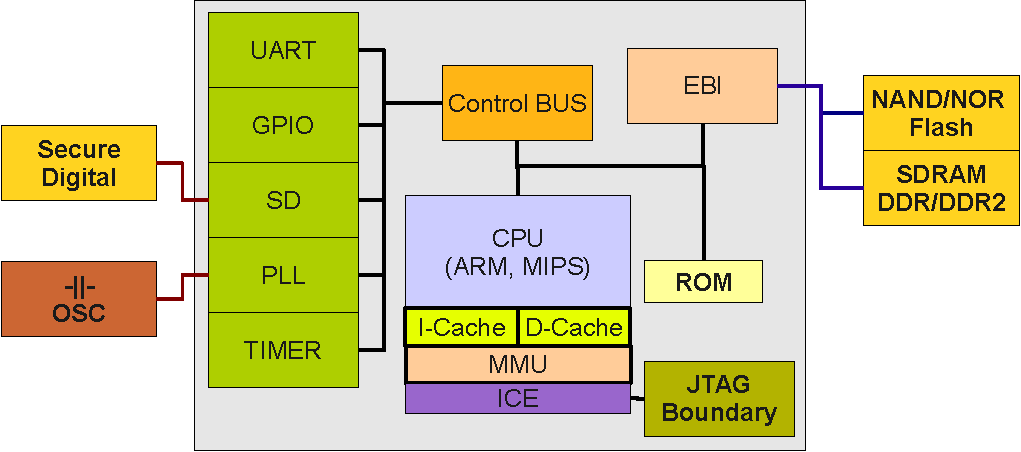
\includegraphics[scale=.45]{../images/soc_no_int_volatil_mmu.pdf} \end{center}
%     };
% 
% 
% 
%     \onslide<3> \node [ph_explain2, right=.5cm of adaptation.east] (exp_adaptation)    
%     {
%     \begin{center} \textbf{Flujo de dise�o Software} \end{center}
%       \begin{center} 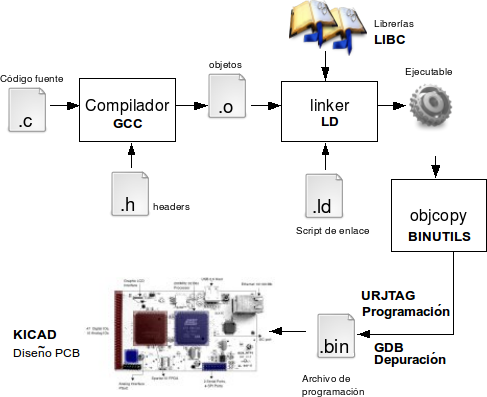
\includegraphics[scale=.6]{../images/SW_design_flow.png} \end{center}
%     };
% 
% 
% 
%     \onslide<4> \node [ph_explain2, right=.2cm of adaptation.east] (exp_adaptation)    
%     {
%     \begin{center} \textbf{Flujo de Dise�o Hardware} \end{center}
%       \begin{center} 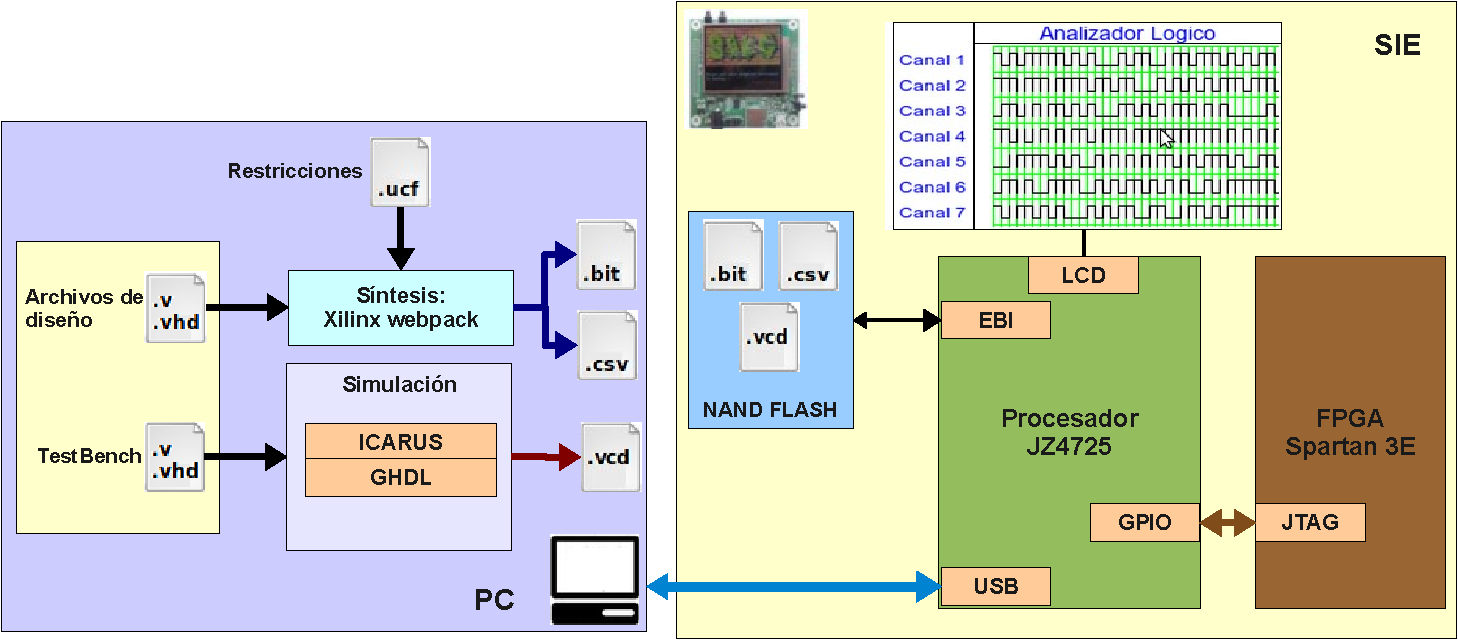
\includegraphics[scale=.37]{../images/HW_design_flow.pdf}   \end{center}
%     };
% 
% 
% 
% 
%     \onslide<5> \node [ph_explain, right=.5cm of adaptation.east] (exp_adaptation)    
%     {
% 
%     \begin{center} \textbf{Flujo de Dise�o SoC (softcore)} \end{center}
% 	\begin{center} 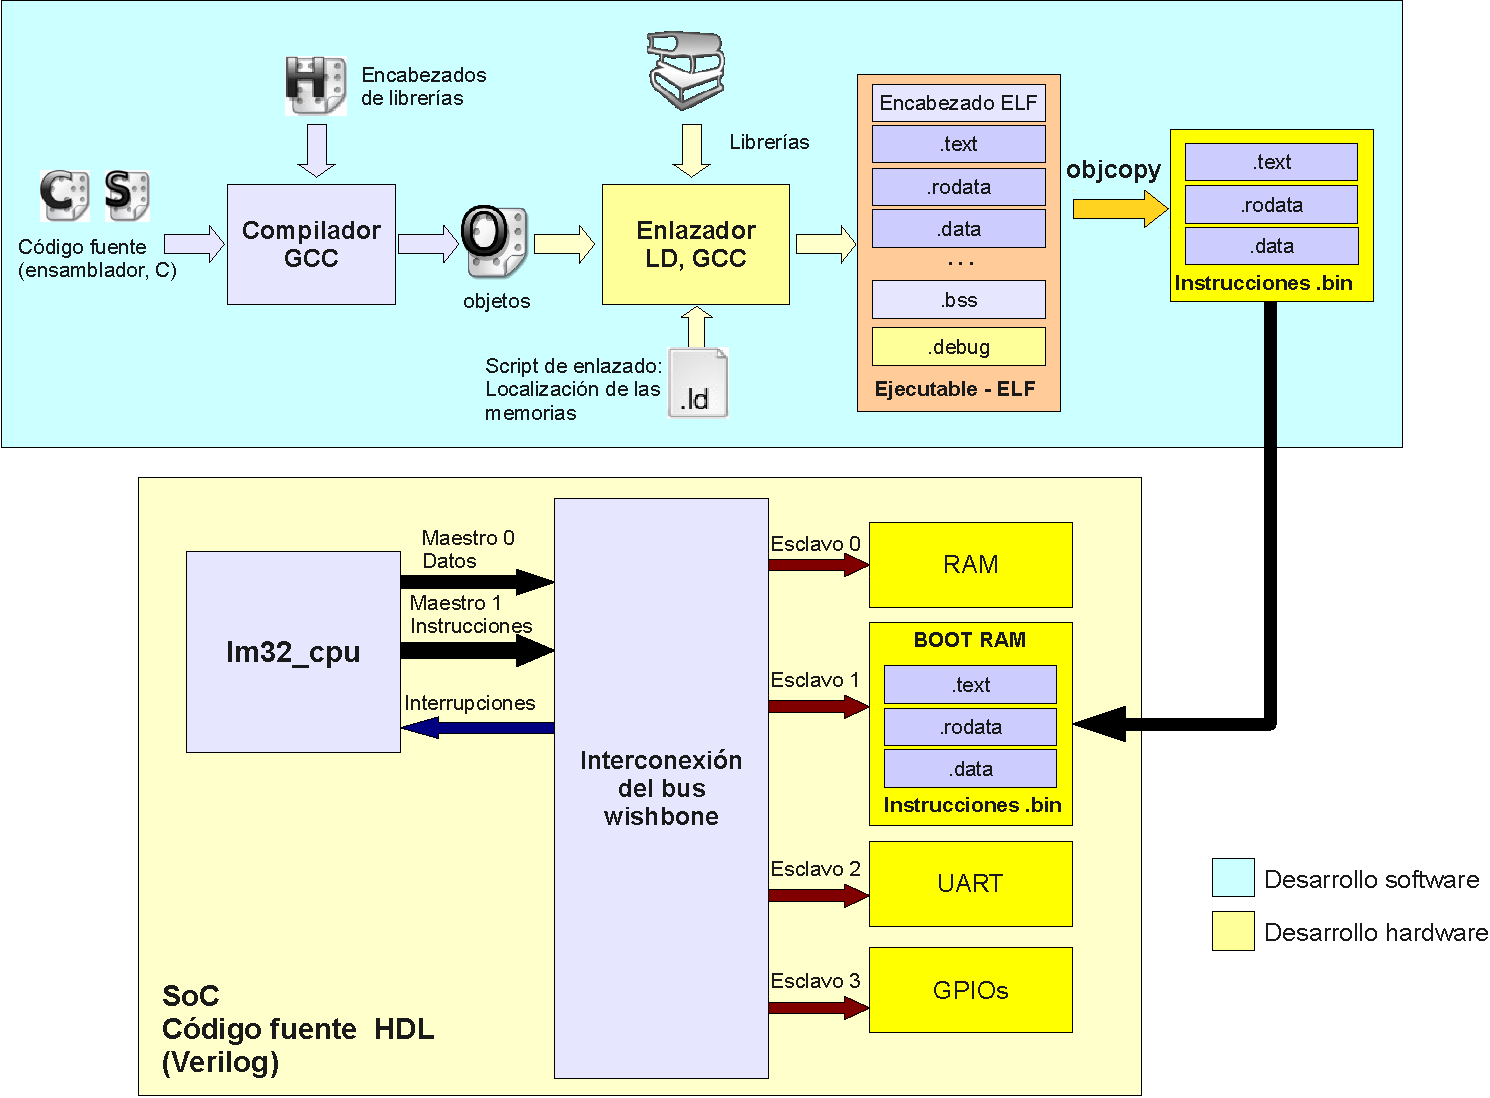
\includegraphics[scale=.35]{../images/soft_SoC_design_flow.pdf}   \end{center}
%     };
% 
%     \onslide<6> \node [ph_explain, right=.5cm of adaptation.east] (exp_adaptation)    
%     {
% %     \begin{center} \textbf{Metodolog�a de dise�o} \end{center}
%         \begin{center} 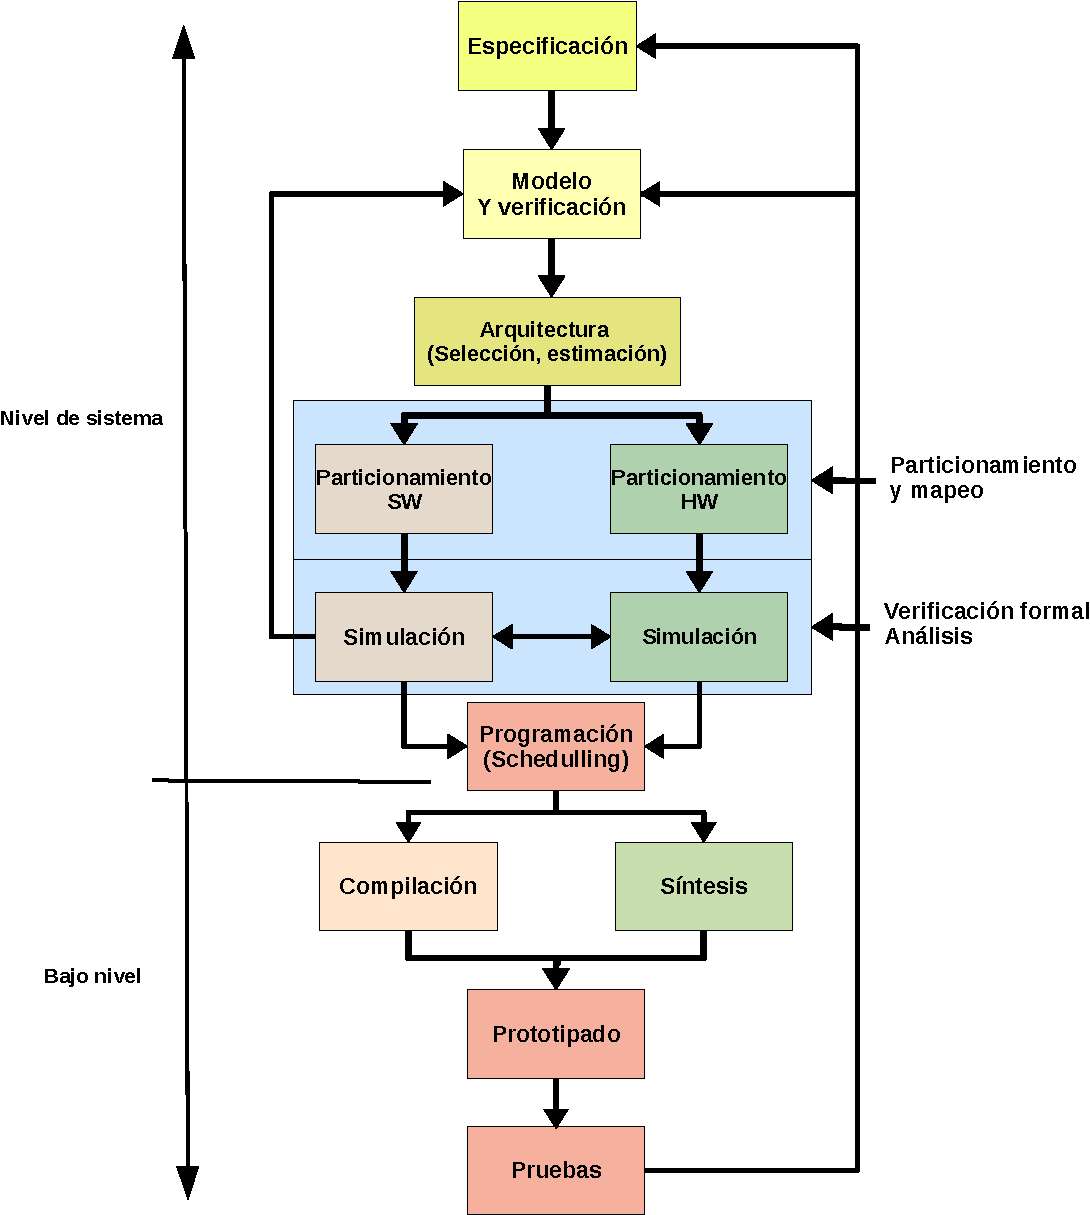
\includegraphics[scale=.45]{../images/embedded_system_design_flow.pdf}   \end{center}
%     };
% 

    \onslide<2> \node [ph_explain2, right=.5cm of adaptation.east] (exp_adaptation)    
    {
    \begin{center} \textbf{Conocimientos adquiridos} \end{center}     

      \begin{itemize}
        \item Metodolog�a para el estudio gradual de la tecnolog�a
        \item Arquitectura de un sistema Embebido. 
        \item Flujo de dise�o software.
        \item Flujo de dise�o hardware.
        \item Flujo de dise�o de SoC (System on a Chip) softcore.
        \item Metodolog�a de dise�o.
        \item Desarrollo de aplicaciones.
          \begin{itemize}
           \scriptsize
           \item Aplicaciones utilizando los sistemas operativos eCos y Linux.
           \item Utilizaci�n de librer�as graficas como QT, Flash.
           \item Creaci�n de sistemas de archivos openwrt, buildroot, openembedded
          \end{itemize}
      \end{itemize}
     
    \begin{center} \textbf{Conocimientos generados} \end{center}     

      \begin{itemize}
        \item Generador de patrones y analizador l�gico utilizando el puerto JTAG.
        \item Drivers para Linux de dispositivos hardware propietarios.
        \item Adaptaci�n del kernel de Linux a nuevas plataformas.
        \item Metodolog�a de ingenier�a inversa.
      \end{itemize}
    };

    
\end{tikzpicture}
\end{figure}

\end{frame}


